\section{Methods}

% ── System Architecture ───────────────────────────────────────────────
\begin{frame}{System Architecture — Four-Layer Stack}
  \centering
  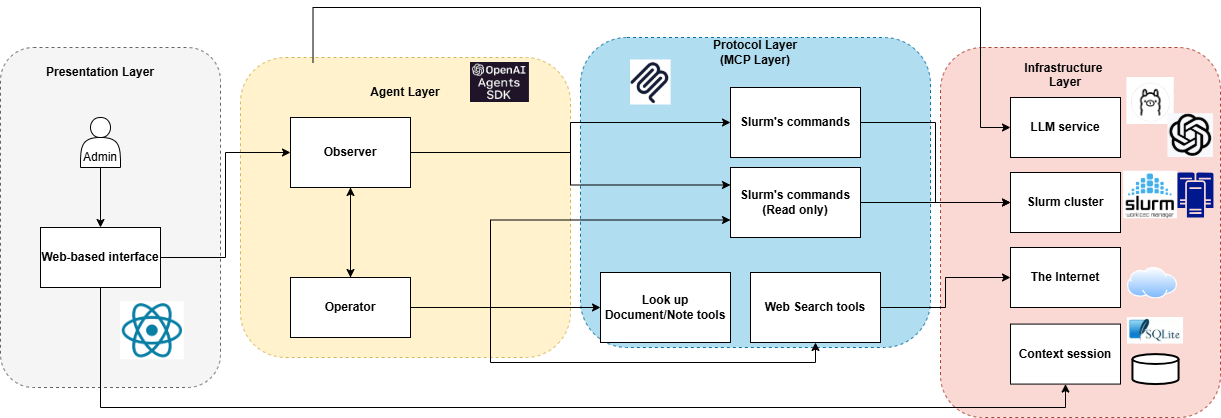
\includegraphics[width=\textwidth]{../report/images/agent_system_architect.drawio.png}
  \captionof{figure}{Presentation → Agent → Protocol (MCP) → Infrastructure}
\end{frame}

% ── Observer / Operator ───────────────────────────────────────────────
\begin{frame}{Observer / Operator Dual-Agent Design}
  \begin{columns}[T]
    \begin{column}{0.64\textwidth}
      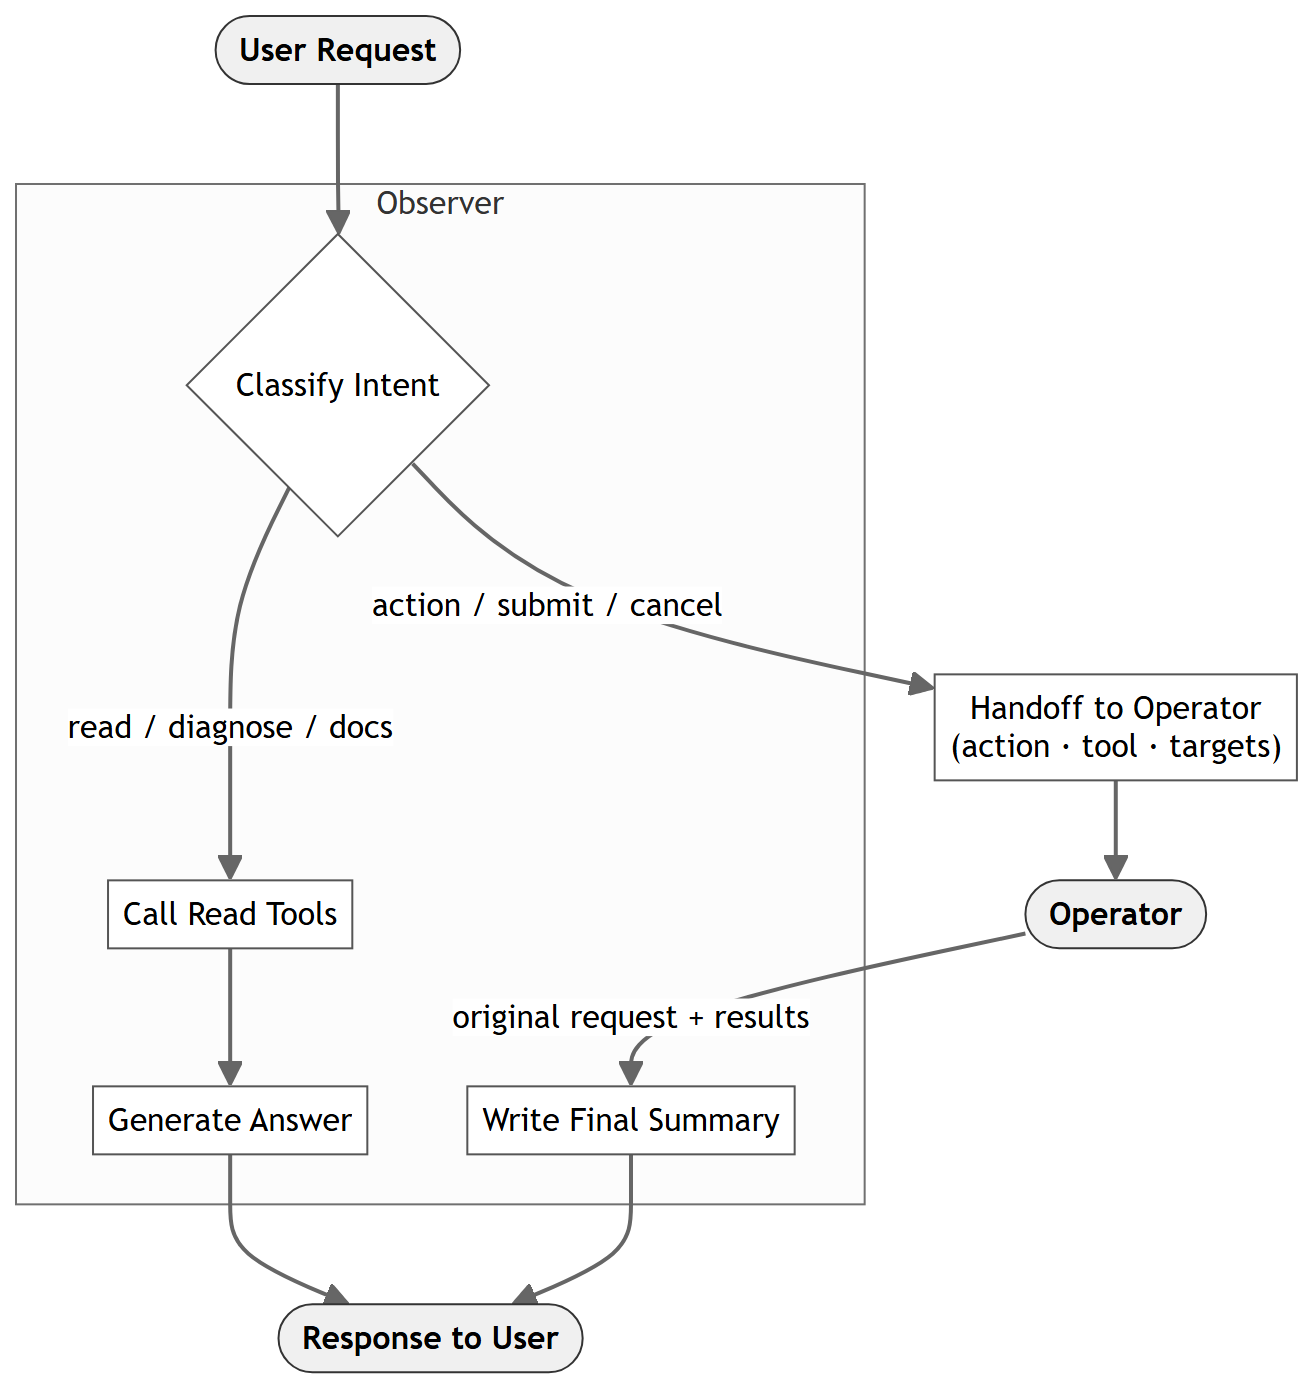
\includegraphics[width=0.49\linewidth, height=5.8cm, keepaspectratio]{../report/images/observer_routing_flow.png}\hfill
      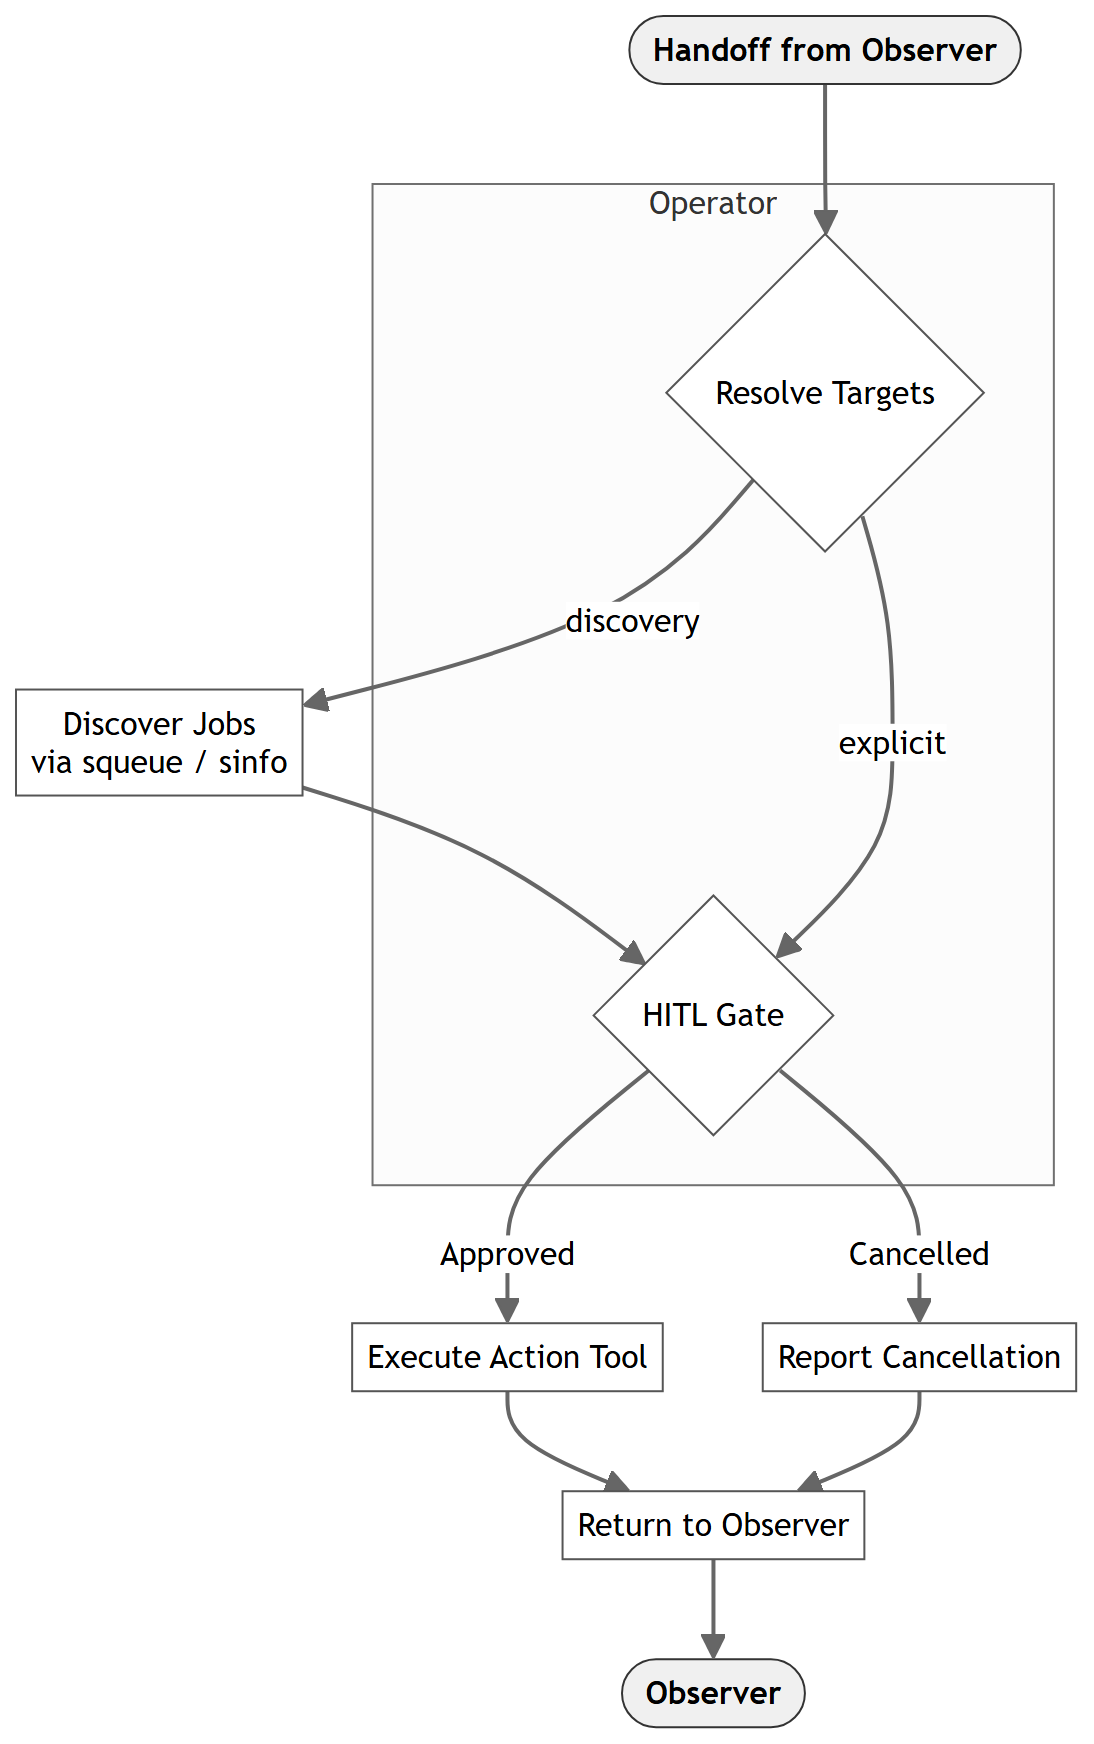
\includegraphics[width=0.49\linewidth, height=5.8cm, keepaspectratio]{../report/images/operator_hitl_flow.png}
      \captionof{figure}{Observer routing (left) and Operator HITL confirmation (right)}
    \end{column}
    \begin{column}{0.33\textwidth}
      \small
      \textbf{Observer} (read-only)
      \begin{itemize}\setlength{\itemsep}{2pt}
        \item 29 read-only tools
        \item Classifies intent; handles monitoring
        \item Issues handoff when mutation needed
      \end{itemize}
      \vspace{0.3em}
      \textbf{Operator} (state-changing)
      \begin{itemize}\setlength{\itemsep}{2pt}
        \item 40 tools (35 action + 5 read)
        \item Receives handoff directive
        \item \textbf{HITL gate} before execution
      \end{itemize}
      \vspace{0.3em}
      Observer \emph{cannot} call \texttt{scancel} — structural safety.
    \end{column}
  \end{columns}
\end{frame}

% ── Tool Partitioning ─────────────────────────────────────────────────
\begin{frame}{Tool Partitioning: Split vs.\ Monolithic}
  \begin{columns}[T]
    \begin{column}{0.48\textwidth}
      \centering
      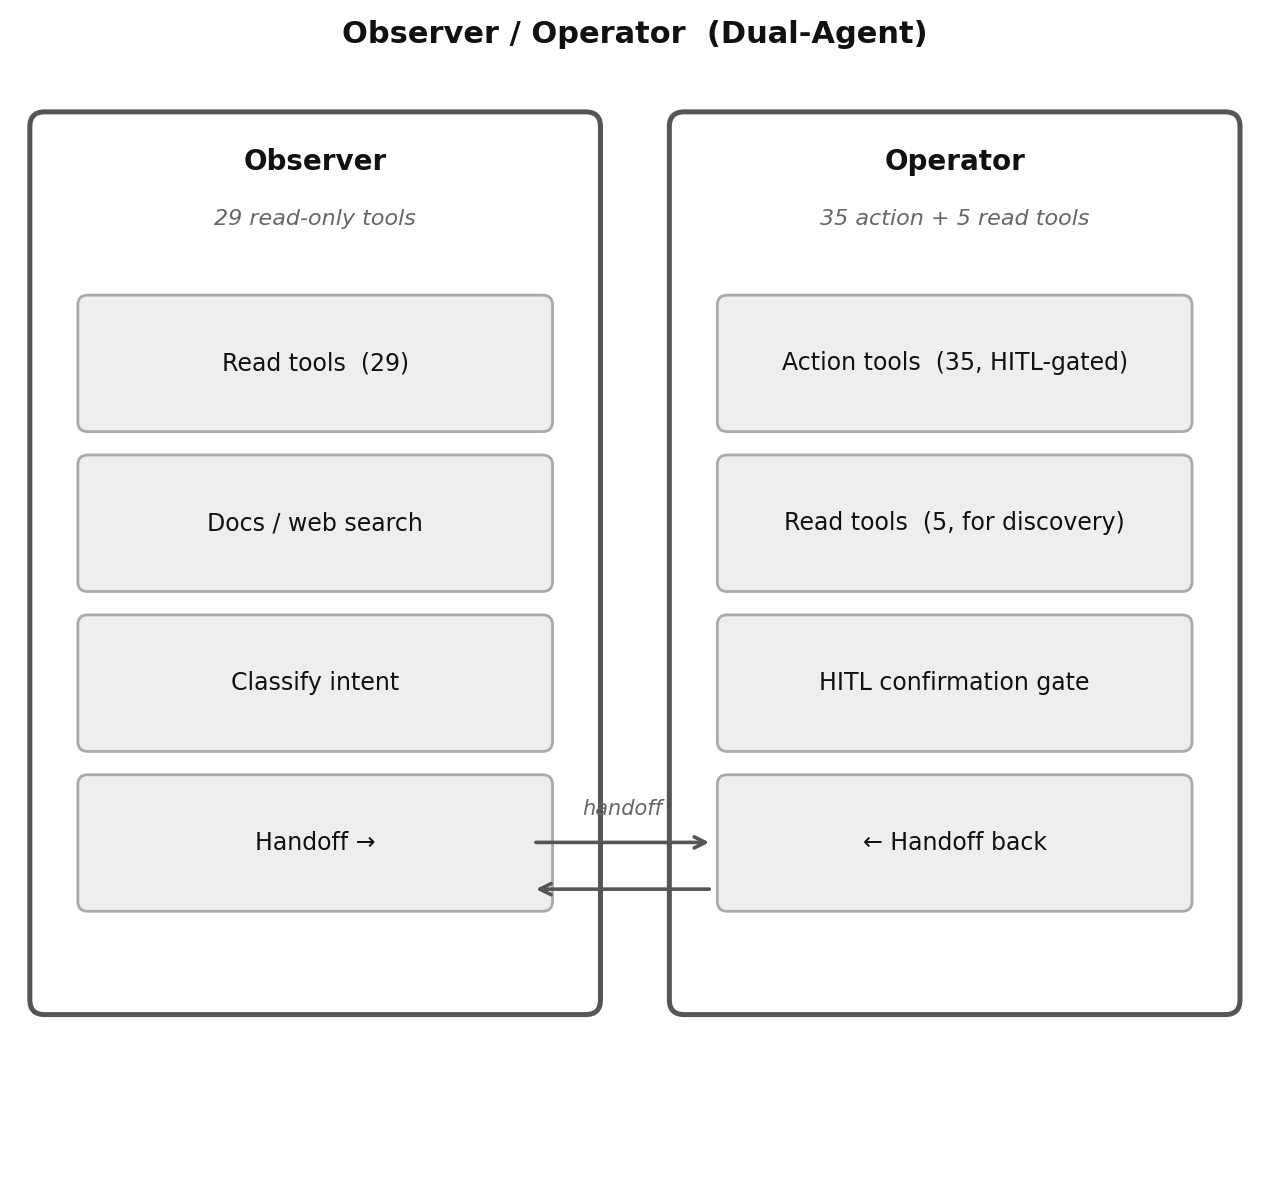
\includegraphics[width=\linewidth, height=5.8cm, keepaspectratio]{../report/images/evaluation/tool_partition_dual.png}
      \captionof{figure}{Observer/Operator split: 29 read-only + 40 tools}
    \end{column}
    \begin{column}{0.48\textwidth}
      \centering
      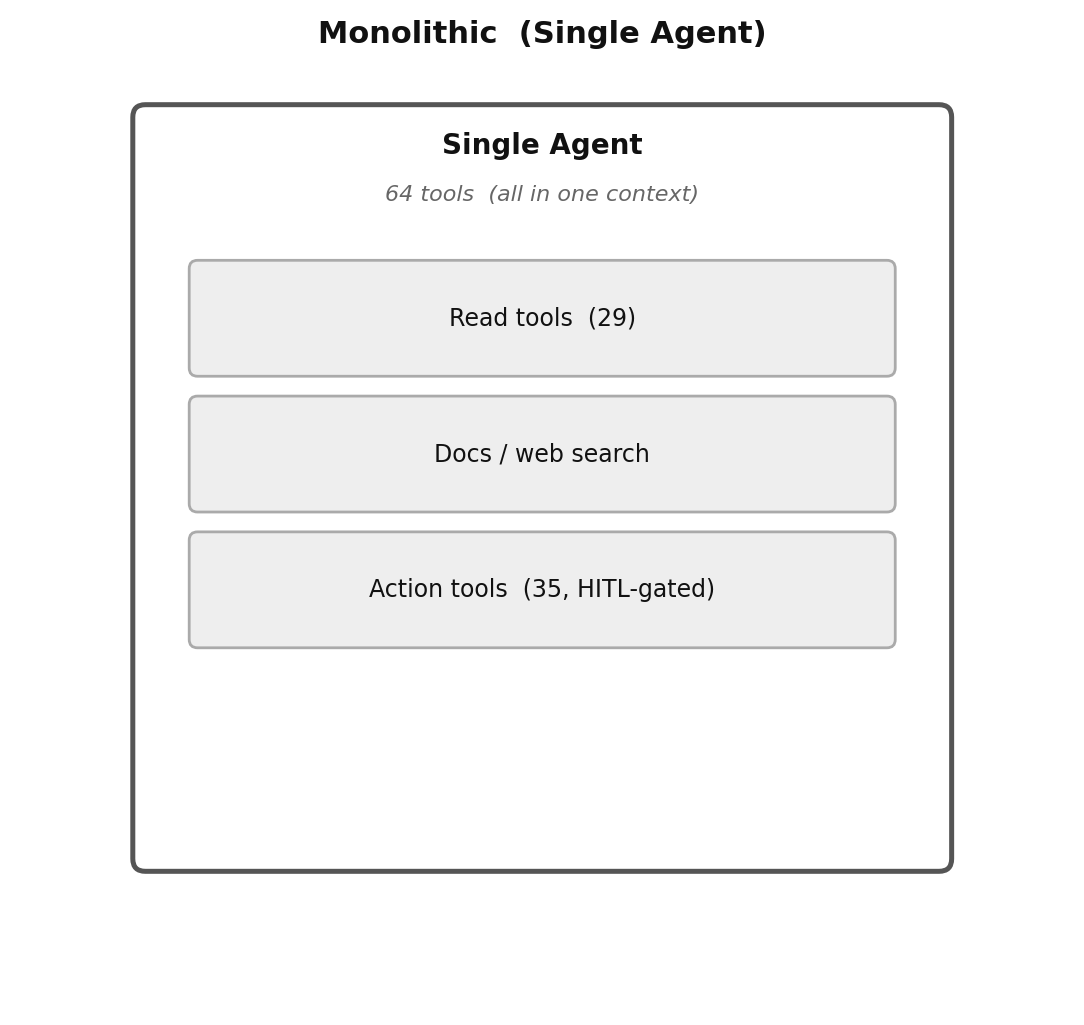
\includegraphics[width=\linewidth, height=5.8cm, keepaspectratio]{../report/images/evaluation/tool_partition_mono.png}
      \captionof{figure}{Monolithic baseline: all 64 tools in one context}
    \end{column}
  \end{columns}
  \vspace{0.3em}
  \centering\small Smaller per-agent context directly improves tool-call accuracy (+7.4\,pp tool recall in ablation).
\end{frame}

% ── MCP Layer ────────────────────────────────────────────────────────
\begin{frame}{MCP Tool Layer}
  \centering
  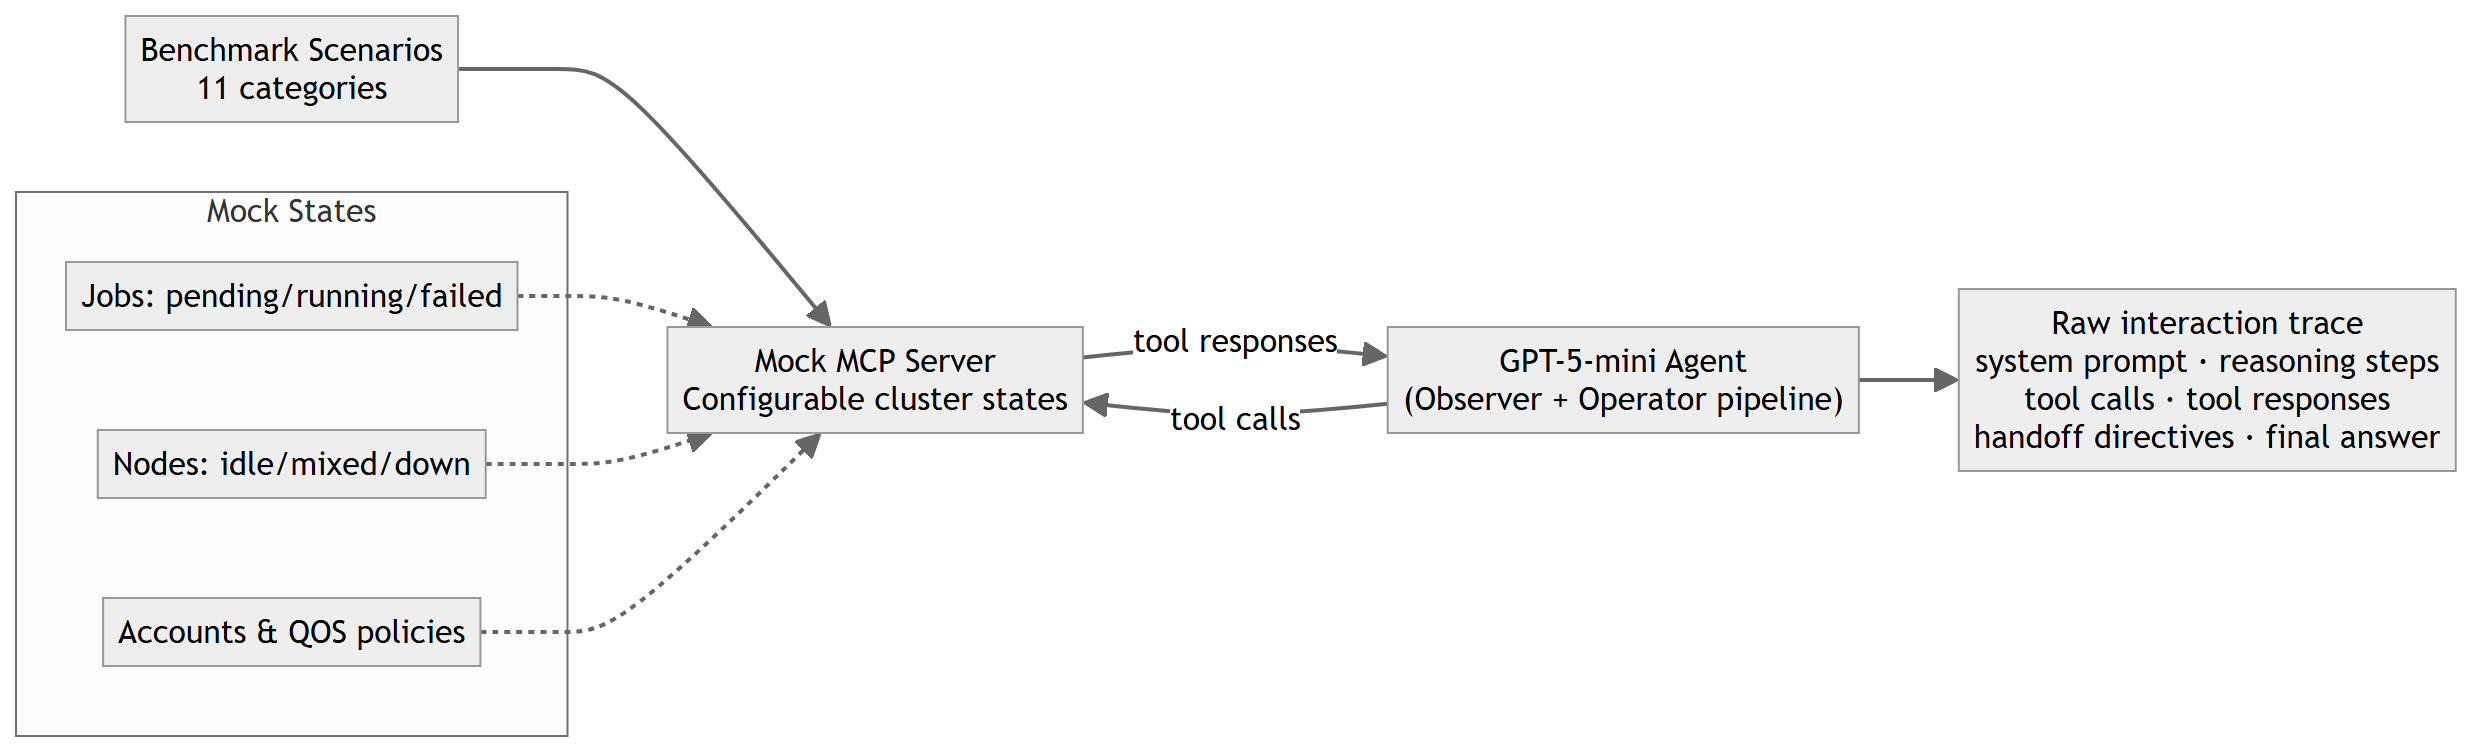
\includegraphics[width=0.92\textwidth, height=6.0cm, keepaspectratio]{../report/images/mcp_mock_data_collection.png}
  \captionof{figure}{MCP tool layer: typed tools, mock engine, trace collection}
  \vspace{0.4em}
  \begin{columns}[T]
    \begin{column}{0.48\textwidth}
      \small\begin{itemize}\setlength{\itemsep}{2pt}
        \item Each Slurm command as a \textbf{typed MCP tool}
        \item Parameter validation — no raw shell
        \item Structured output for model consumption
      \end{itemize}
    \end{column}
    \begin{column}{0.48\textwidth}
      \small\begin{itemize}\setlength{\itemsep}{2pt}
        \item Same layer for real Slurm \& mock engine
        \item \textbf{64 tools}: queue, nodes, accounting, QoS, submission, control, admin, docs
      \end{itemize}
    \end{column}
  \end{columns}
\end{frame}

% ── Training Data Prep ───────────────────────────────────────────────
\begin{frame}{Training Data Preparation}
  \begin{columns}[T]
    \begin{column}{0.48\textwidth}
      \centering
      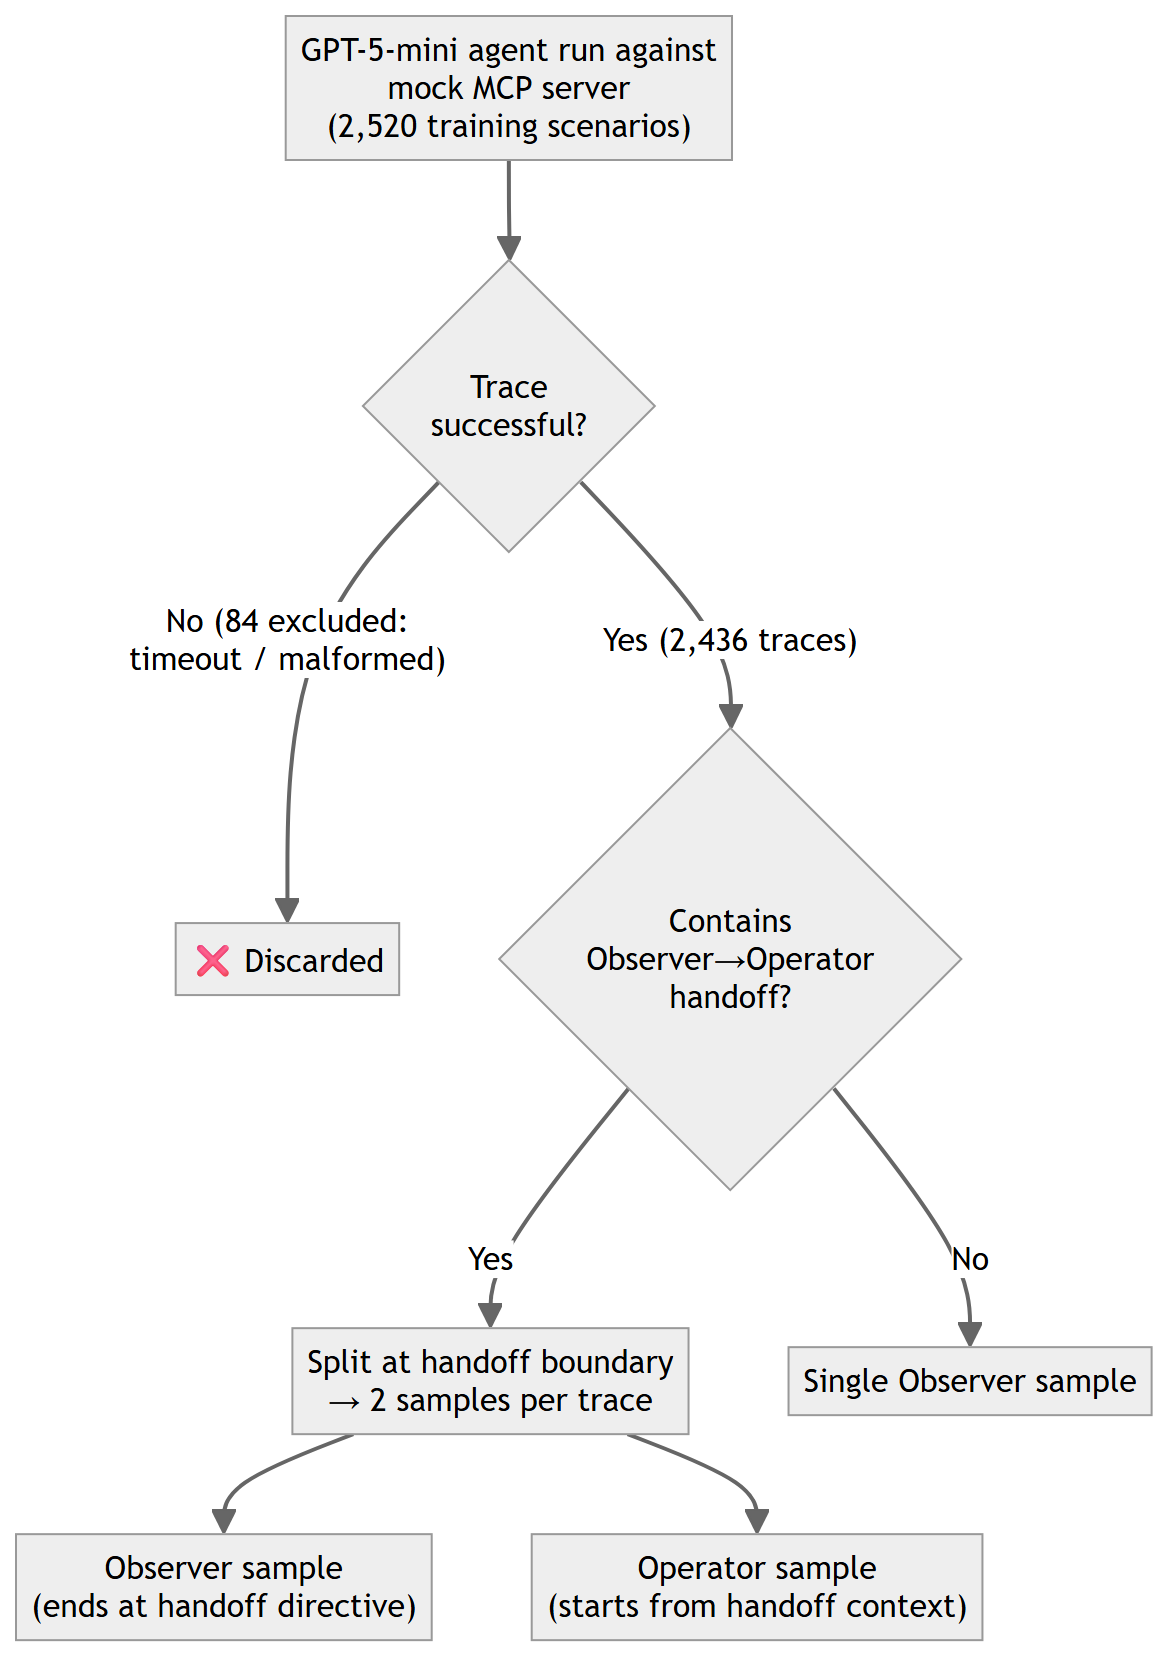
\includegraphics[width=\linewidth, height=6.5cm, keepaspectratio]{../report/images/data_augmentation_phase1.png}
      \captionof{figure}{\textbf{Phase 1:} GPT-5-mini traces role-split at handoff boundary}
    \end{column}
    \begin{column}{0.48\textwidth}
      \centering
      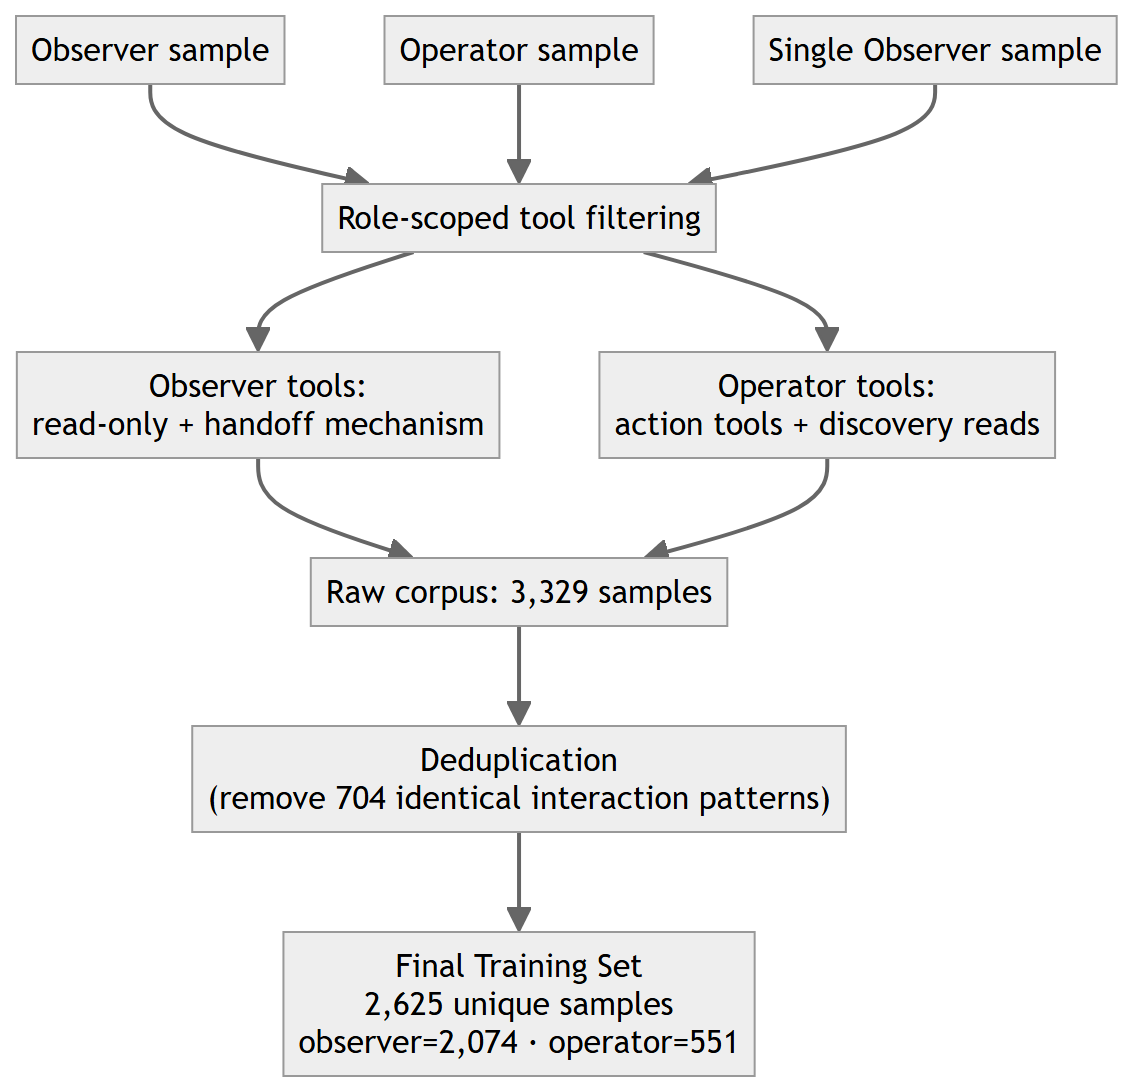
\includegraphics[width=\linewidth, height=6.5cm, keepaspectratio]{../report/images/data_augmentation_phase2.png}
      \captionof{figure}{\textbf{Phase 2:} Role-scoped filtering + dedup $\to$ 2,625 samples}
    \end{column}
  \end{columns}
\end{frame}

% ── QLoRA Fine-Tuning ────────────────────────────────────────────────
\begin{frame}{Domain Adaptation: QLoRA Fine-Tuning}
  \begin{columns}[T]
    \begin{column}{0.48\textwidth}
      \textbf{Model setup}
      \begin{itemize}\setlength{\itemsep}{6pt}
        \item Base: Qwen2.5-14B-Instruct
        \item 4-bit NF4 quantization, all 48 layers
        \item LoRA r=64, $\alpha$=128 — \textbf{275M trainable params} (1.9\%)
        \item bfloat16 adapters, 8,192 token context
        \item Loss on assistant tokens only
      \end{itemize}
    \end{column}
    \begin{column}{0.48\textwidth}
      \textbf{Training}
      \begin{itemize}\setlength{\itemsep}{6pt}
        \item 2,625 distilled GPT-5-mini traces
        \item Role-scoped tool lists per sample
        \item 3 epochs, lr=1e-4, cosine schedule
        \item Effective batch 16 (grad accum $\times$16)
        \item $\sim$22\,h on a single A40 (48\,GB)
      \end{itemize}
    \end{column}
  \end{columns}
\end{frame}
